\section{در این تمرین قصد داریم تا پردازنده‌های سیستم‌عامل لینوکس را مورد بررسی قرار دهیم}

اولین دستوری که می‌خواهیم بررسی کنیم، دستور \texttt{ps} است.این دستور اطلاعات پردازه‌ها را نمایش می‌دهد.
\begin{qsolve}[خروجی دستور \texttt{ps}]
	\begin{center}
		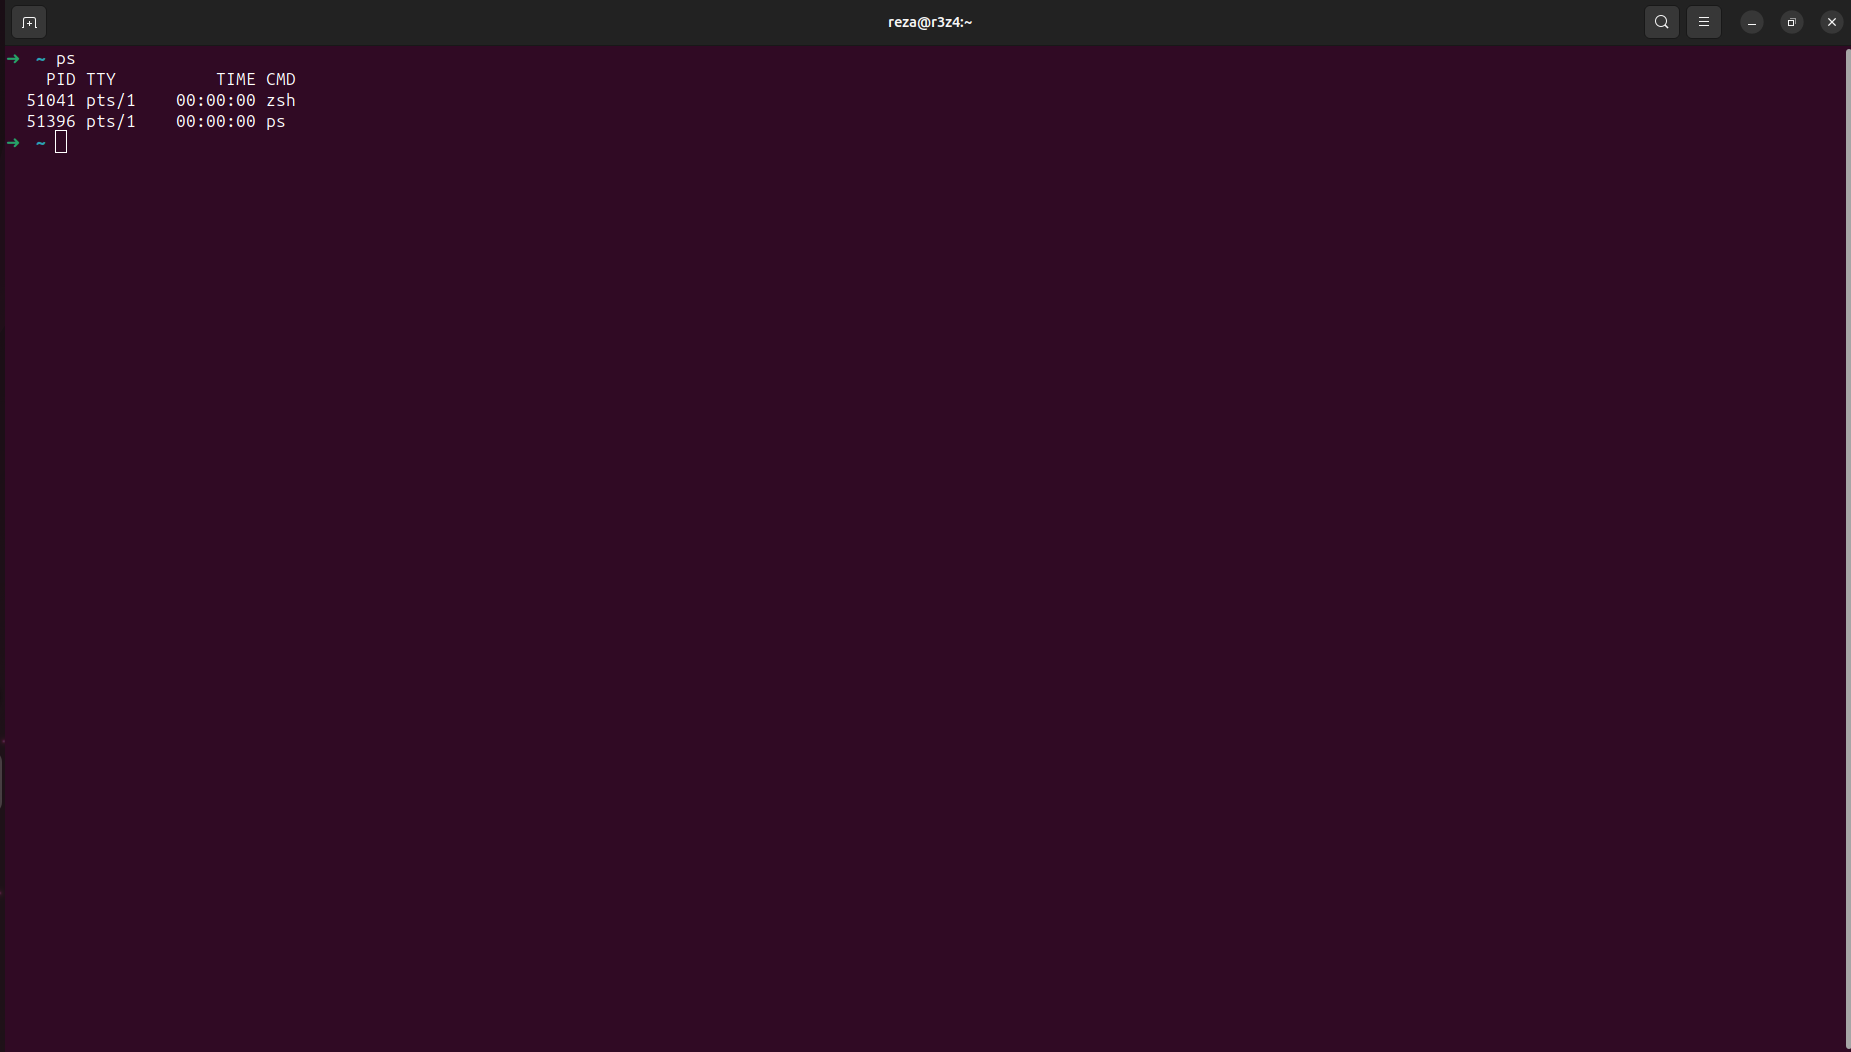
\includegraphics[width=\textwidth]{pics/img1.png}
	\end{center}
\end{qsolve}

برای درک وضعیت فعلی فرآیند‌های درحال اجرای سیستم خود، دستور \texttt{aux ps} بیشترین مقدار اطلاعاتی که یک کاربر معمولا نیاز دارد را نمایش می‌دهد.

در خروجی این دستور وضعیت هر پردازه (Stat) و شماره هر پردازه (PID) و سایر اطلاعات موجود است.

شماره پردازه‌ها در خروجی دستور \texttt{ps} از ۱ شروع شده و می‌دانیم که یک پردازه جدید در سیستم‌عامل با استفاده از دستورات \texttt{fork} و \texttt{exec} ساخته می‌شود. بنابراین هر پردازه ای یک پردازه والد دارد.

برای یافتن شماره پردازه والد، می‌توان از دستور \texttt{[pid] -f ps} استفاده کرد. این دستور \texttt{PPID} که شماره پردازه والد هست را نیز نمایش می‌دهد. از این دستور استفاده کنید و پردازه والد پردازه ۱ را پیدا کنید.

دستور \texttt{[pid] -P pgrep} همه فرزندان یک پردازه را نمایش می‌دهد. از این دستور استفاده کنید و همه پردازه‌هایی که پردازه پدر مشترکی با پردازه ۱ دارند را پیدا کنید.

همچنین با استفاده از دستور \texttt{pstree} می‌توان ارتباط بین پردازه‌ها را نمایش داد.



\begin{qsolve}[خروجی دستور \texttt{aux ps}]
	\begin{center}
		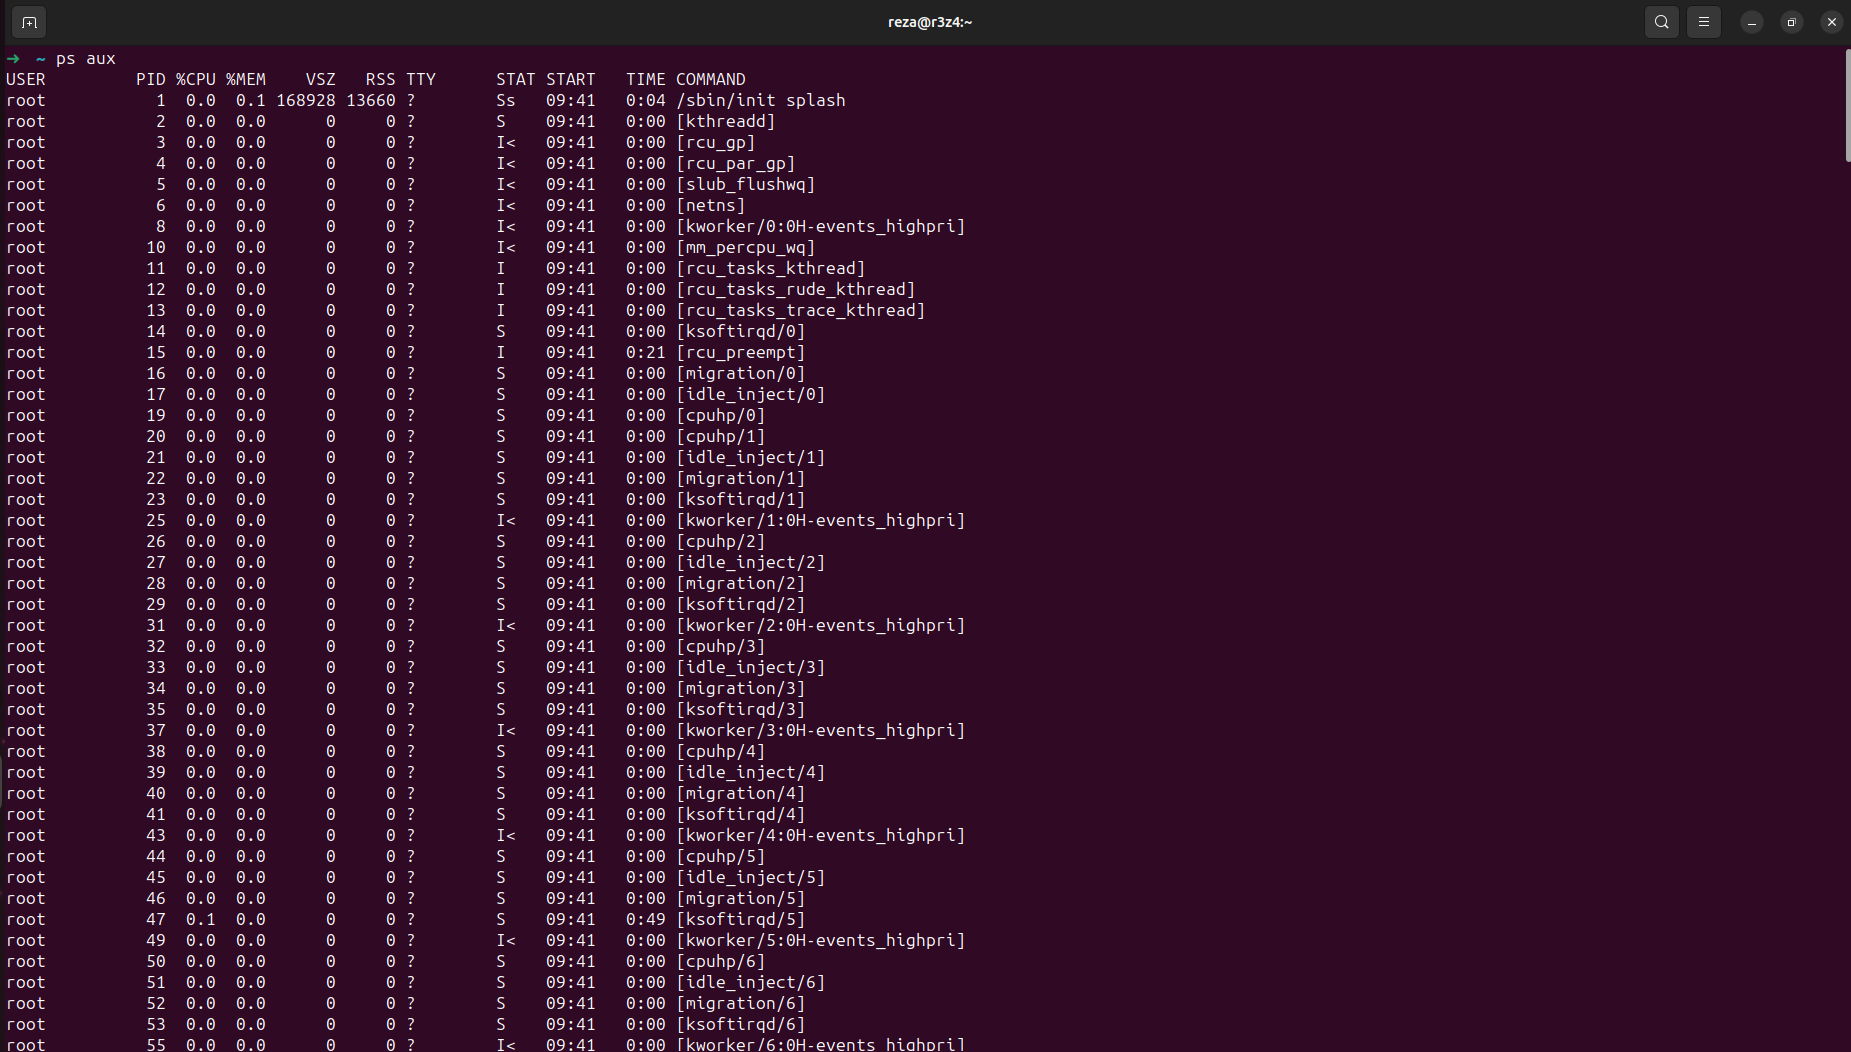
\includegraphics[width=\textwidth]{pics/img2.png}
	\end{center}
\end{qsolve}

\begin{qsolve}[خروجی دستور \texttt{[pid] -f ps}]
	\begin{center}
		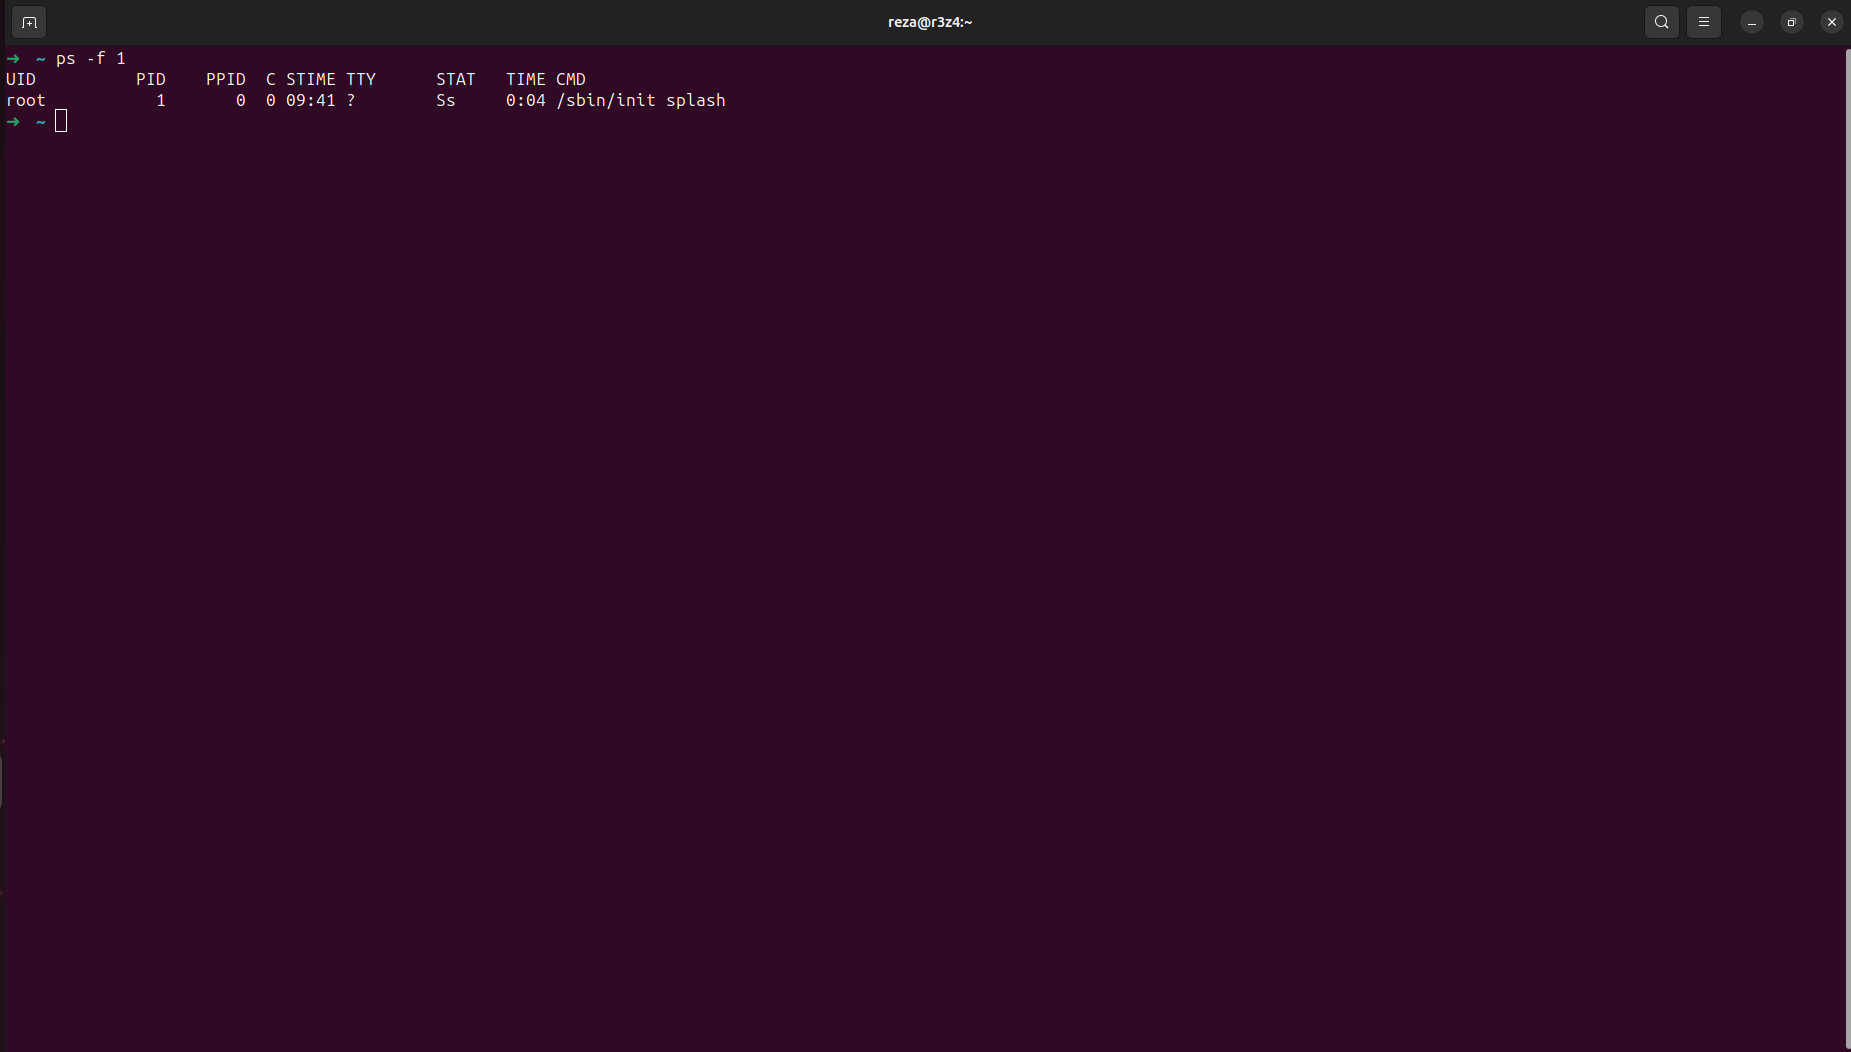
\includegraphics[width=\textwidth]{pics/img3.png}
	\end{center}
\end{qsolve}

\begin{qsolve}[خروجی دستور \texttt{[pid] -P pgrep}]
	\begin{center}
		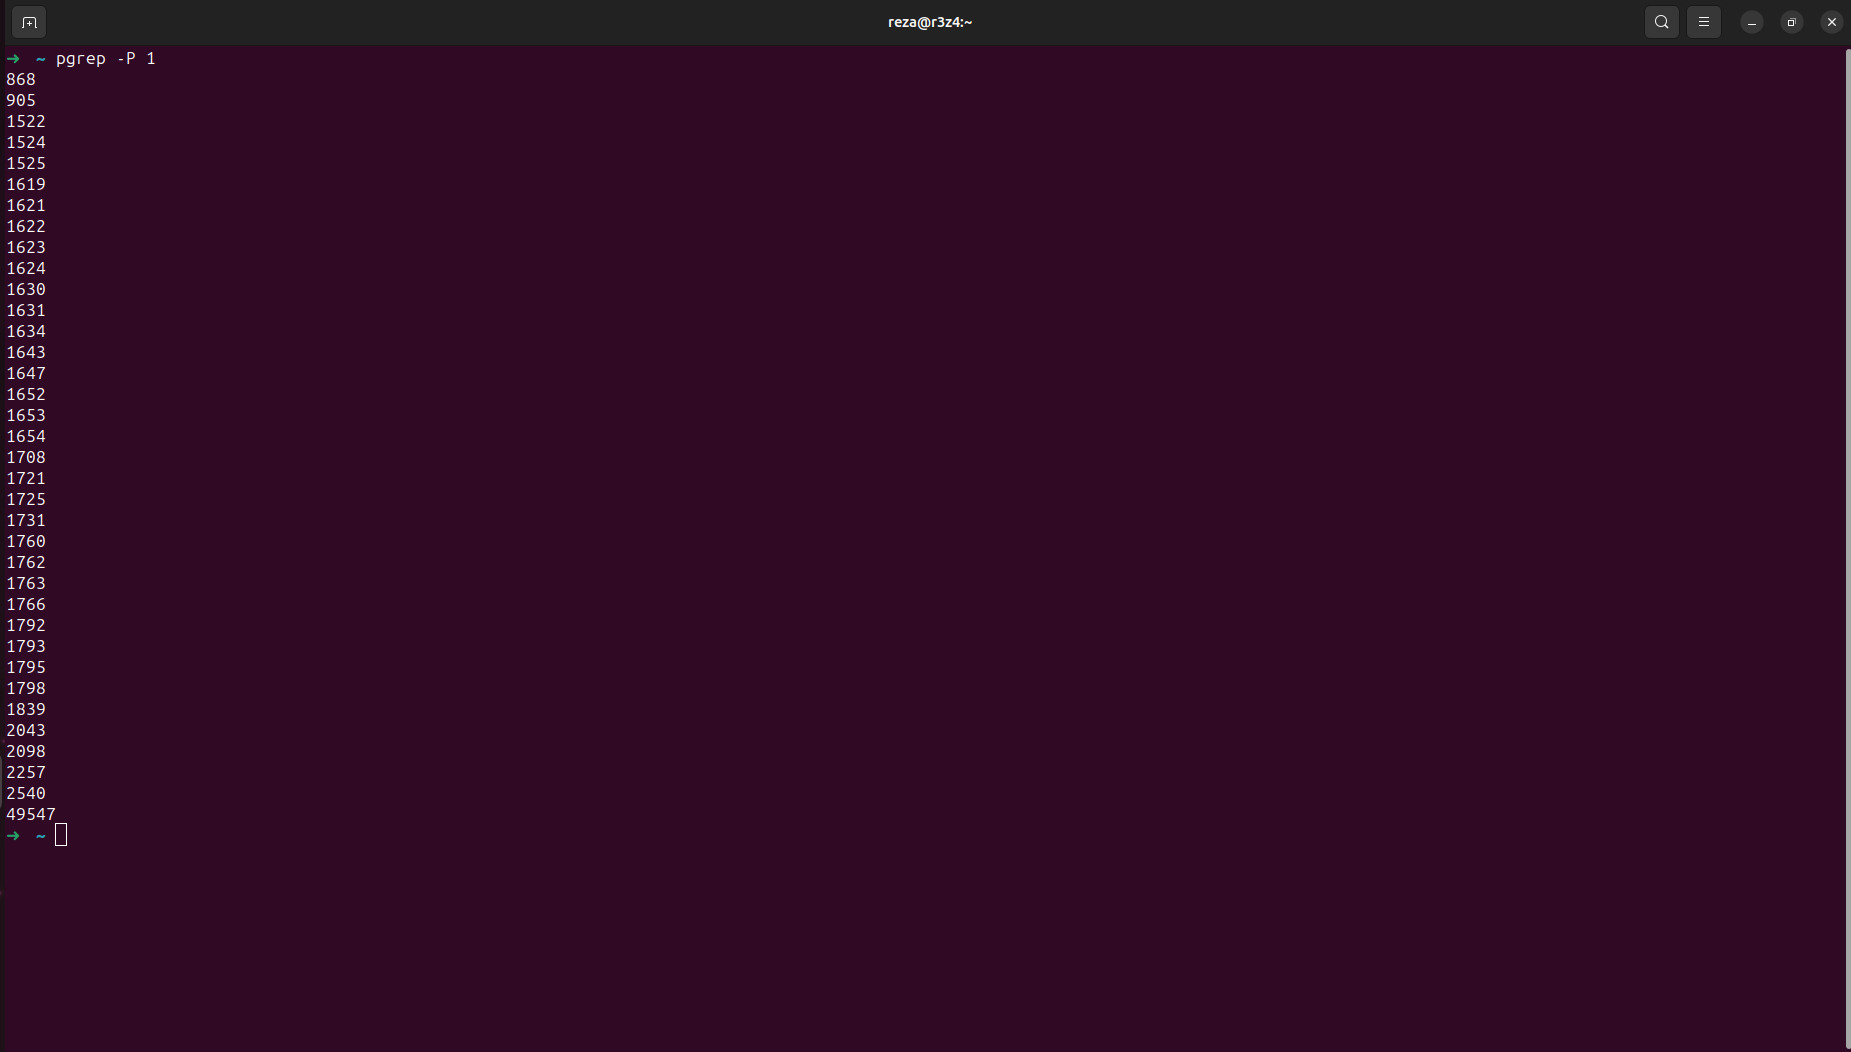
\includegraphics[width=\textwidth]{pics/img4.png}
	\end{center}
\end{qsolve}

\begin{qsolve}[خروجی دستور \texttt{pstree}]
	\begin{center}
		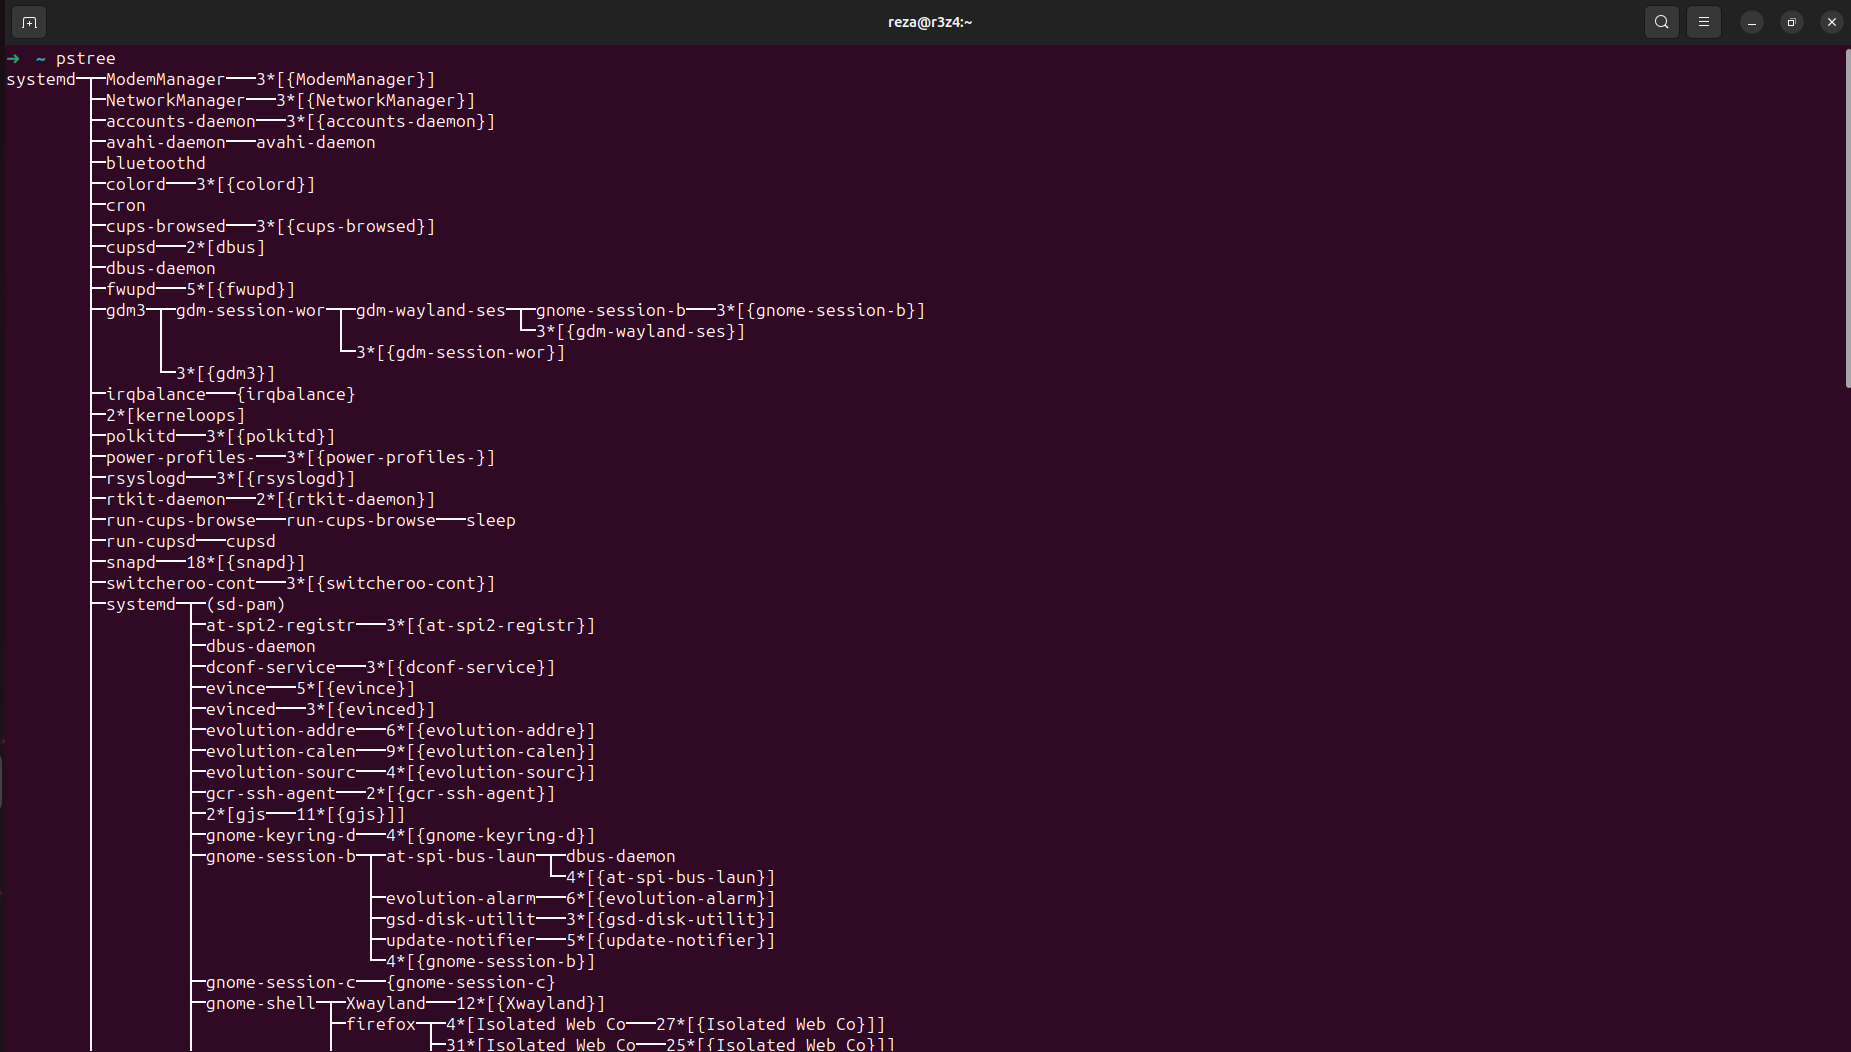
\includegraphics[width=\textwidth]{pics/img5.png}
	\end{center}
\end{qsolve}
